
\subsection{Inputs}

\colorlet{shadecolor}{Mycolor3}
\begin{shaded}
\subsubsection{Fuel ($w$)}
The framework will use a measure of fractional cover as a proxy for fuel continuity (i.e, annual mean or maximum fAPAR, as used by \citet{knorr2014impact,knorr2016climate} or MODIS fractional cover). \citet{bistinas2014causal} uses SeaWiFs fAPAR, but this product was discontinued in 2005, so would reduce our comparison period. Other fAPAR/Fractional cover products would probably cover a larger period.
\end{shaded}
\colorlet{shadecolor}{Mycolor2}

\begin{figure}[!ht]
  \centering
    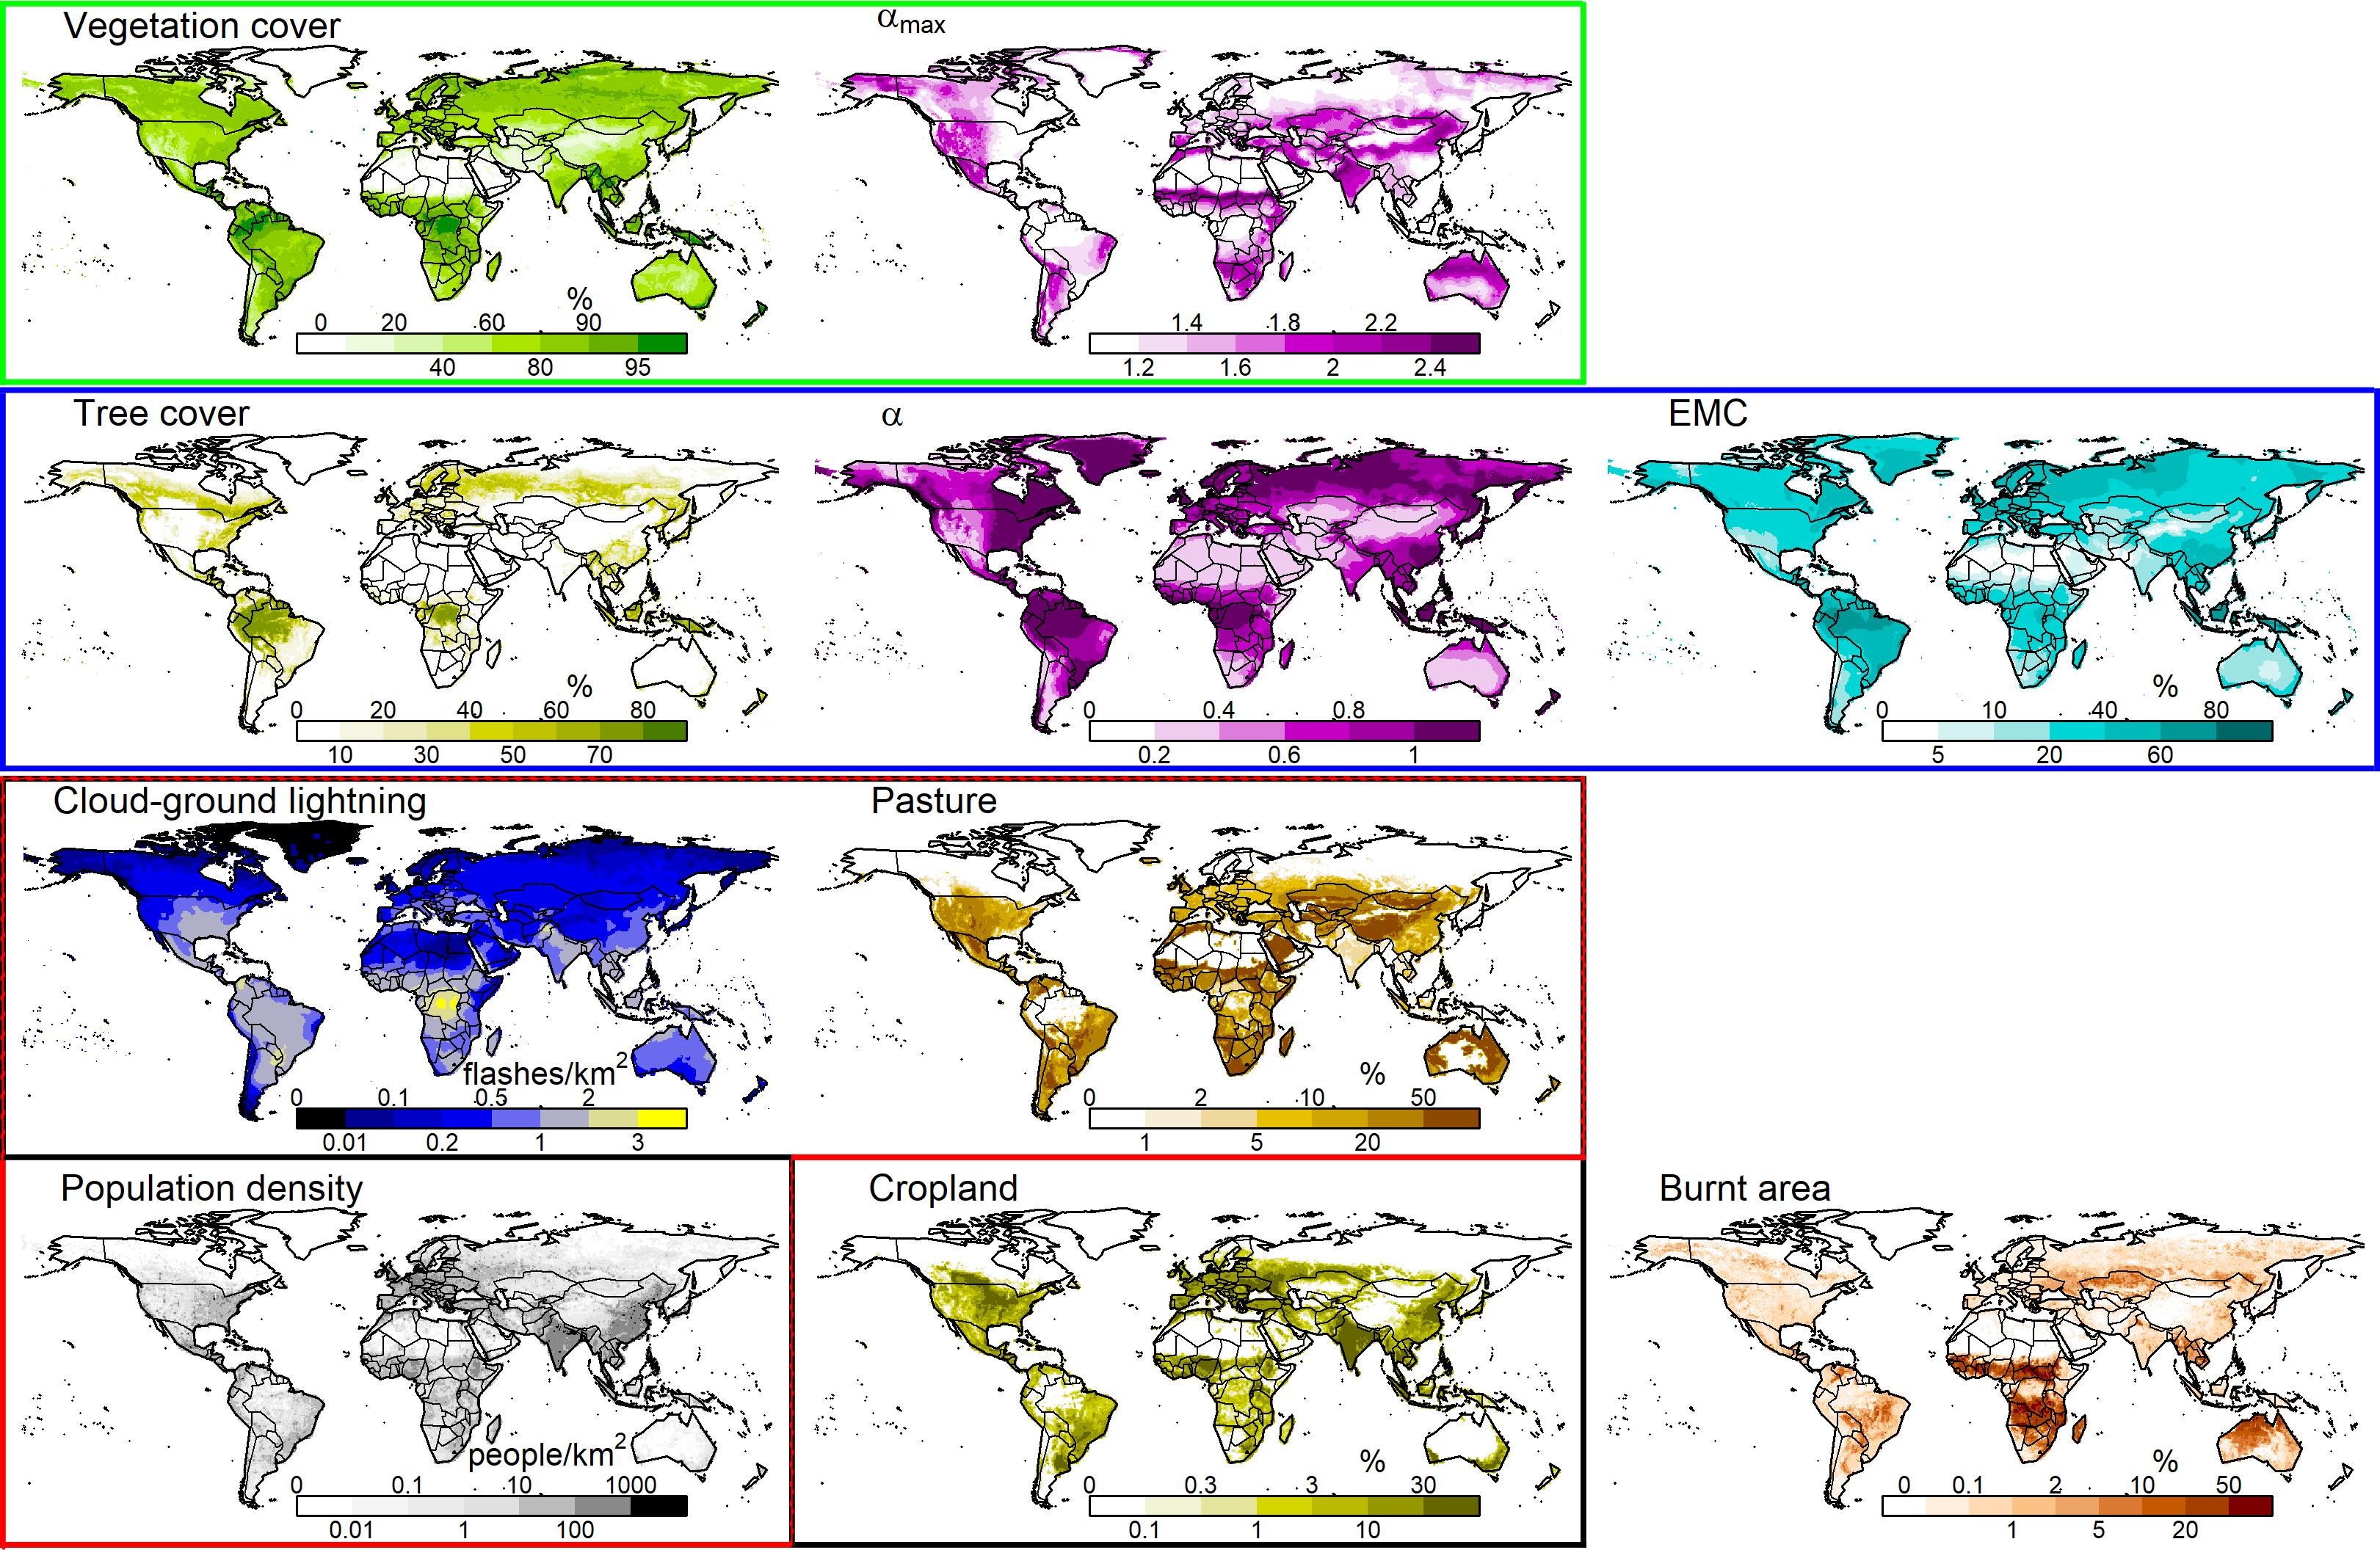
\includegraphics[width=0.67\textwidth]{../figs/inputs_mean.pdf}
  \caption{Monthly means of each framework input \hlr{add units} and GFEDv4.}
  \label{fig:Monthly_mean_ins}
\end{figure}

\begin{figure}[!ht]
  \centering
    \includegraphics[width=0.67\textwidth]{../figs/inputs_fireSeason.pdf}
  \caption{Monthly means during the fire season for each input \hlr{add units} and GFEDv4 training data. ``Fire season'' is defined as the month with heighest burnt area, calculated each year.}
  \label{fig:Season_mean_ins}
\end{figure}

\begin{figure}[!ht]
  \centering
    \includegraphics[width=0.67\textwidth]{../figs/input_correlation.pdf}
  \caption{Input correlations.}
  \label{fig:Corr_ins}
\end{figure}

\subsubsection{Moisture ($\omega$)}

$\omega$ represents mean fractional water content of fuel, and combines contributions from soil (i.e from live fuels - $\alpha$) and atmopshere ($atm$) coupling:

\begin{equation}
    \omega = (\alpha + M \cdot atm) / (1 + M)
\end{equation}

where $M$ is an optimised parameter, representing the relative importance of atmospheric to soil coupling.

\paragraph{Soil-coupled contribution.}
The ratio of actual to potential evaporation \citep[$\alpha$][]{prentice1993simulation}, a measure of available soil water in relation to plant demand, is used to describe fractional water content soil-coupled fuels as per \citet{harrison2010fire, bistinas2014causal}.
$\alpha$ is calculated from CRUTS3.22 monthly mean temperature, cloud cover and precipitation using the STASH model \citep{sykes1996bioclimatic} r-package \citep{rstash}. \hlb{At the moment, elevation, is set to zero and field capacity to 140 - Rhys, I guess this will have to change? Any suggestions for data?}. STASH was spun up by recycling 1950 climate data for 40 years and then run from 1950 to 2010. Simulated $\alpha$ from 2000-2010 used for the rest of the analysis.

\begin{shaded}
\paragraph{Atmosphere-controlled} ($atm$) could be represented using either STASH outputs or by a simple equilibrium moisture content calculation ($m_{mq}$).
\begin{itemize}

\item \textbf{STASH}. The ratio of condensation rate ($Con$) and atmospheric evaportaive demand (i.e $PET$) could be used to calculate ``fuel drying speed'' ($FDS$):

    \begin{equation}
        FDS = \frac{Con}{PET}
    \end{equation}
    here, when $FDS>1$, daily condensation occurs more rapidly than drying, and fuel load mositure will increase, and when $FDS<1$, fuel drys faster then condenstation and fuel moisture will decrease. \\
    \\
    There are a few things to consider here:

    \begin{enumerate}
        \item How should precip be included? Options are to add it to the $Con$ term:

        \begin{equation}
            FDS = \frac{Con + Pr}{PET}
        \end{equation}
        \\
        \\
        or give FDS a maximum value of 1, which is also equivilent to a wetday:

        \begin{equation}
            FDS = WD + (1 - WD) \cdot \min(1, Con/PET)
        \end{equation}
        where $WD$ is fractional wet days
        \\
        \\
        or something else

        \item Is PET being double counted (I couldnt quiet get my head round this bit). If so, there could be a way of combininbg soil and atmopshere:

        \begin{equation}
            \omega_{*} = \frac{AET + C_n}{PET}
        \end{equation}
        \\
        \\
        or maybe

        \begin{equation}
            \omega_{*} = \frac{AET}{PET - C_n}
        \end{equation}
        \\
        \\
        which could also be combined with rainfall:

        \begin{equation}
            \omega = WD + (1 - WD) \cdot min(1, \omega_{*})
        \end{equation}

    \end{enumerate}

    \item $m_{mq}$ is currently used and is calculated from \citep{viney1991review} which combines daily precipitaion ($Pr$) and atmopheric drying potential via temprature ($T$) and relative humidity ($H_r$):

    \begin{equation}
         m_{mq, daily}=
            \begin{cases}
                10 - (T - H_r) / 4 ,& \text{if } Pr\leq 3 \text{mm}\\
                100,              & \text{otherwise}
            \end{cases}
    \end{equation}
    On a monthly timestep, this simplifies to:

    \begin{equation}
         m_{mq}=
            (10 - (T - H_r) / 4) \cdot (1 - WD)
            + 100 \cdot WD
    \end{equation}
    where WD is the monthly fraction of wet days from CRU TS3.22, where a wetday is defined as a day where $Pr > 3mm$. $H_r$ was calculated as the ratio of actual to saturated vapour pressure \hlb{ref??}:

    \begin{equation}
        H_r = 100 \cdot AVP / SVP
    \end{equation}
    monthly $AVP$ is from CRUTS.22. $SVP$ was calculated from mean monthly temperature as per \citet{walter2000asce}

    \begin{equation}
        SVP = 6.11 \cdot 10^{\frac{7.5 \cdot T}{237.5 + T}}
    \end{equation}


    %calculates daily condenstation rates , expressed as the water-equivalent of daily negative net surface radiation:

    %\begin{equation}
    %        C_n = E_{con} \cdot |H^{*}_N| \times 10^3
    %\end{equation}

\end{itemize}

\end{shaded}

\subsubsection{Igntions ($ig$)}

Ignition combines sources from lightning ($L_{ig}$), pasture and the local population.

\begin{equation}
    ig = L_{ig} + P \cdot Pasture + D \cdot Population\text{ }Density
\end{equation}
where P and D are optimized parameters.

\begin{shaded}
    We could also add background igntions:

    \begin{equation}
        ig = 1 + N \cdot L_{ig} + P \cdot Pasture + D \cdot Population\text{ }Density
    \end{equation}
    where N, P and D are opimized paramters describing the contribution of their respective ignition source relative to background igntions.
\end{shaded}


\begin{figure}[!ht]
  \centering
    \includegraphics[width=0.67\textwidth]{../figs/measure_mean.pdf}
  \caption{Monthly means of each control. \hlr{add units?}}
  \label{fig:Monthly_mean_controls}
\end{figure}

\begin{figure}[!ht]
  \centering
    \includegraphics[width=0.67\textwidth]{../figs/measure_fire.pdf}
  \caption{Monthly means of each control during the fire season. \hlr{add units?}}
  \label{fig:Season_mean_controls}
\end{figure}

\paragraph{Lightning}
is calculated from
from the Lightning Imaging Sensor flash count climatology (LIS \cite{christian1999lightning}, http://grip.nsstc.nasa.gov/). \hlb{Are there other products that could be used instead?}
This product contains both cloud-to-ground ($CG$ - available for ignition) and inter-cloud (not available for ignitions) strikes.
$CG$ lighting is calculated using \citet{kelley2014improved}:

\begin{equation}
    L_{ig} = FL * min(1, 0.0408 \cdot FL^{-0.4180})
\end{equation}
where FL is the flash count recorded by LIS over a 0.5 degree cell.

\paragraph{Pasture and population density}
\label{Pasture}
are taken from the HYDE dataset \citep{klein2007mapping}, and are interpolated from a decadal to a monthly timestep.

\subsubsection{Supression ($s$)}

Suppression combines urban and cropland area and population density

\begin{equation}
    s = urban + C \cdot Crop + H \cdot Population\text{ }Density
    \label{equ:Supression}
\end{equation}

where $C$ and $H$ are optimised parameters.

\textbf{Urban} and \textbf{cropland} areas are taken from HYDE and processed as per pasture and population desnity (section ~\ref{Pasture})


\begin{figure}[!ht]
\colorlet{shadecolor}{Mycolor3}
\begin{shaded}
  \centering
    \includegraphics[width=0.67\textwidth]{../figs/limitation_lines.png}

  \caption{Limitation contribution for each control.}
  \label{fig:lim_lines}
\end{shaded}
\colorlet{shadecolor}{Mycolor2}

\end{figure}
